% *********************************************************************
% © 2016–2019 Jeremy Sylvestre
%
% Permission is granted to copy, distribute and/or modify this document
% under the terms of the GNU Free Documentation License, Version 1.3 or
% any later version published by the Free Software Foundation; with no
% Invariant Sections, no Front-Cover Texts, and no Back-Cover Texts. A
% copy of the license is included in the appendix entitled “GNU Free
% Documentation License” that appears in the output document of this
% PreTeXt source code. All trademarks™ are the registered® marks of
% their respective owners.
%
% *********************************************************************
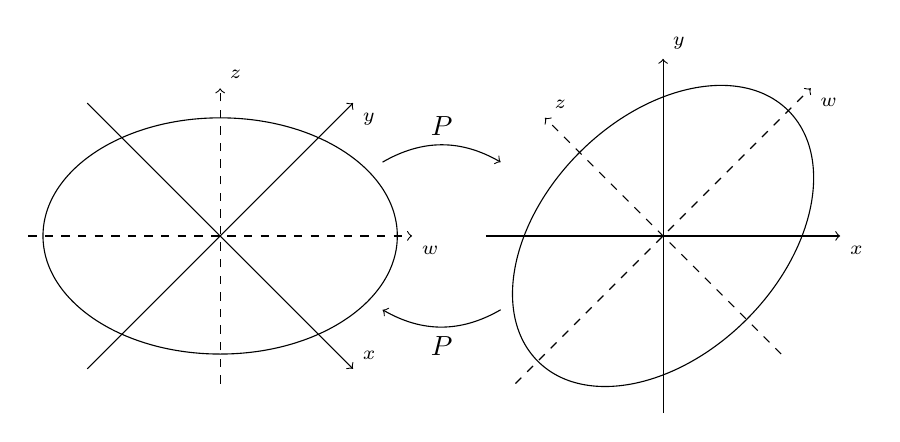
\begin{tikzpicture}[
	point/.style={circle,draw,very thin,fill,inner sep=0pt,minimum size=4pt},
	vector/.style={-latex},
	scale=0.75,
]

	\begin{scope}[xshift=7.5cm]

		\draw[->] (-3,0) to (3,0) node[below right] {$\scriptstyle x$};
		\draw[->] (0,-3) to (0,3) node[above right] {$\scriptstyle y$};

		\draw[dashed,->] (2,-2) to (-2,2) node[above right] {$\scriptstyle z$};
		\draw[dashed,->] (-2.5,-2.5) to (2.5,2.5) node[below right] {$\scriptstyle w$};

		\draw[rotate=45] (0,0) ellipse (3cm and 2cm);

	\end{scope}

	\draw[dashed,->] (-3.25,0) to (3.25,0) node[below right] {$\scriptstyle w$};
	\draw[dashed,->] (0,-2.5) to (0,2.5) node[above right] {$\scriptstyle z$};
	\draw[->] (-2.25,2.25) to (2.25,-2.25) node[above right] {$\scriptstyle x$};
	\draw[->] (-2.25,-2.25) to (2.25,2.25) node[below right] {$\scriptstyle y$};

	\draw (0,0) ellipse (3cm and 2cm);

	\draw[->] (2.75,1.25) to [out=30,in=150] node[above] {$P$} (4.75,1.25);
	\draw[->] (4.75,-1.25) to [out=-150,in=-30] node[below] {$\inv{P}$} (2.75,-1.25);

\end{tikzpicture}
